%From https://egu2018.eu/PICO_how-to_guide_to_PICO.pdf
%Abstracted and templated by Brian Ballsun-Stanton, Macquarie University.
%original template by https://github.com/snowtechblog/pico-latex-presentation by Anselm Köhler


%Pico on faims 3
%Slide 1: 
%	Dataapp challenge precis
%	Pictures from different workflows
%Slide 2:
%	How we solve it
%	Our winning pitch in pictures
%Section 2:
%	Our pitch in more pictures, highlights our OSS plans and what OSS components we plan to reuse.
%Section 3:
%	How CSIRO would use our pitch.





\documentclass[unknownkeysallowed,usepdftitle=false, parskip=full, t]{beamer}
% unknownkeysallowed is needed for mac and the newer latex version -> is more picky than before...
\usetheme[headheight=1cm,footheight=2cm]{boxes}
%\usetheme{default}


\usepackage{default}
\usepackage{graphicx}
%example pictures created via: http://lorempixel.com/1200/800/cats/Figure2/. Credit to http://lorempixel.com/images.php

\usepackage{epsfig}
\usepackage{siunitx}
\usepackage{color}
\usepackage{ifthen}
%usepackage{ragged2e}

\usepackage{natbib}



\usepackage[T1]{fontenc}
\usepackage[utf8]{inputenc}
%https://tex.stackexchange.com/a/203804/5483

\makeatletter
\renewcommand{\itemize}[1][]{%
  \beamer@ifempty{#1}{}{\def\beamer@defaultospec{#1}}%
  \ifnum \@itemdepth >2\relax\@toodeep\else
    \advance\@itemdepth\@ne
    \beamer@computepref\@itemdepth% sets \beameritemnestingprefix
    \usebeamerfont{itemize/enumerate \beameritemnestingprefix body}%
    \usebeamercolor[fg]{itemize/enumerate \beameritemnestingprefix body}%
    \usebeamertemplate{itemize/enumerate \beameritemnestingprefix body begin}%
    \list
      {\usebeamertemplate{itemize \beameritemnestingprefix item}}
      {\def\makelabel##1{%
          {%
            \hss\llap{{%
                \usebeamerfont*{itemize \beameritemnestingprefix item}%
                \usebeamercolor[fg]{itemize \beameritemnestingprefix item}##1}}%
          }%
        }%
      }
  \fi%
  \beamer@cramped%
  %\justifying% NEW
  %\raggedright% ORIGINAL
  \beamer@firstlineitemizeunskip%
}
\makeatother


\usepackage[activate={true,nocompatibility},final,tracking=true,kerning=true,spacing=true,factor=1100,stretch=10,shrink=10]{microtype}
\SetExtraKerning[unit=space]
    {encoding={*}, family={bch}, series={*}, size={footnotesize,small,normalsize}}
    {\textendash={400,400}, % en-dash, add more space around it
     "28={ ,150}, % left bracket, add space from right
     "29={150, }, % right bracket, add space from left
     \textquotedblleft={ ,150}, % left quotation mark, space from right
     \textquotedblright={150, }} % right quotation mark, space from left
 % http://www.khirevich.com/latex/microtype/
\microtypecontext{spacing=nonfrench}

\usepackage{lipsum} % for dummy text only
\usepackage[UKenglish]{babel} %https://tex.stackexchange.com/a/27743 
\usepackage[pangram]{blindtext} % https://tex.stackexchange.com/a/48411

%\usepackage{parskip} % from https://tex.stackexchange.com/q/11622
%\setlength{\parskip}{12pt} 

%\setparsizes{\parindent}{12pt}{\parfillskip}

%\usepackage{etoolbox} % as per https://tex.stackexchange.com/a/24331
%\appto\chapterheadendvskip{\vspace{-1\parskip}}
%\setparsizes{\parindent}{50pt plus 20pt minus 30pt}{\parfillskip}

\setbeamertemplate{navigation symbols}{}%remove navigation symbols
\setbeamersize{text margin left=1cm,text margin right=1cm}

% some colors
\definecolor{grau}{gray}{.5}
\definecolor{slfcolor}{rgb}{0,0.6274,0.8353}
\definecolor{wslcolor}{rgb}{0,0.4,0.4}

% setup links
\hypersetup{%
	%linkbordercolor=green,%
	colorlinks=false,%
	pdfborderstyle={/S/U/W 0},%
	%pdfpagemode=FullScreen,%
	pdfstartpage=4%
	}

% setup some fonts
\setbeamerfont{title}{series=\bfseries, size*={9pt}{0pt}}
\setbeamerfont{author}{size*={4.5pt}{0pt}}
\setbeamerfont{institute}{size*={2.5pt}{0pt}}
\setbeamerfont{bodytext}{size=\scriptsize}
	
% Title setup	
\title{FAIMS Mobile 3.0: A next-generation field data collection platform}
\author{Brian Ballsun-Stanton\inst{1} (\texttt{brian.ballsun-stanton@mq.edu.au})  Shawn Ross\inst{1}  Steve Cassidy\inst{1} Nathan Reid\inst{2}  Jens Klump\inst{2}}
\institute{\inst{1}Macquarie University, Sydney, Australia
\quad \inst{2}Mineral
Resources, CSIRO, Kensington WA, Australia}
% add title in headbox
\setbeamertemplate{headline}
{\leavevmode
\begin{beamercolorbox}[width=1\paperwidth]{head title}
{\vspace{0.1cm}}
  % LOGO
  \begin{columns}[t, totalwidth=\textwidth]
  \begin{column}[c]{1.1cm}
     \hskip0.1cm 
\includegraphics[width=1cm]{figure/mq.jpg}
  \end{column}
  % TITLE
   \begin{column}[c]{10.3cm}
   \centering \usebeamerfont{title} \textcolor{slfcolor}{\inserttitle} \\
   \centering \usebeamerfont{author} \color[rgb]{0,0,0} \insertauthor \\
   \vspace{-0.05cm}
   \centering \usebeamerfont{institute} \insertinstitute
  \end{column}
  % PICTURE
  \begin{column}[c]{1.1cm}
    
    
\includegraphics[width=1cm]{figure/csiro.jpg}\hspace{0.2cm}
  \end{column}
  \end{columns}
  {\color{slfcolor}\hrule height 1pt}
\end{beamercolorbox}%
}

% setup the navigation in footbox
% first set some button colors
\newcommand{\buttonactive}{\setbeamercolor{button}{bg=wslcolor,fg=white}}
\newcommand{\buttonpassive}{\setbeamercolor{button}{bg=slfcolor,fg=black}}
% now set up that the one active one gets the new color.
\newcommand{\secvariable}{nothing}
% therefore we write before each section (well, everything which should be part of the navi bar)
% the variable \secvariable to any name which is in the next function ...
\newcommand{\mysection}[1]{\renewcommand{\secvariable}{#1}
}
% ... compaired to strings in the following navibar definition ...
\newcommand{\tocbuttoncolor}[1]{%
 \ifthenelse{\equal{\secvariable}{#1}}{%
    \buttonactive}{%
    \buttonpassive}
 }
% ... here we start to set up the navibar. each entry is calling first the function \tocbuttoncolor with the argument which should be tested for beeing active. if active, then change color. afterwards the button is draw. so to change that, you need to change the argument in \toc..color, the first in \hyperlink and before each frames definition... A bit messed up, but works...
\newlength{\buttonspacingfootline}
\setlength{\buttonspacingfootline}{-0.2cm}
\setbeamertemplate{footline}
{\leavevmode
\begin{beamercolorbox}[width=1\paperwidth]{head title}
  {\color{slfcolor}\hrule height 1pt}
  \vspace{0.05cm}
  % set up the buttons in an mbox
  \centering \mbox{
    \tocbuttoncolor{madness}
    \hyperlink{madness}{\beamerbutton{2 Minute Madness}}
    \tocbuttoncolor{challenge}
    \hspace{\buttonspacingfootline}
      \hyperlink{challenge}{\beamerbutton{DataApp Challenge}}

    \tocbuttoncolor{solution}
    \hspace{\buttonspacingfootline}
      \hyperlink{solution}{\beamerbutton{Proposed Solution}}
    \tocbuttoncolor{oss}
    \hspace{\buttonspacingfootline}
      \hyperlink{oss}{\beamerbutton{OSS Technologies}}
    \tocbuttoncolor{CSIRO}
    \hspace{\buttonspacingfootline}
      \hyperlink{CSIRO}{\beamerbutton{CSIRO's plans}}
    
    
    % this last one should normaly not be used... it will open the preferences to change the 
    % behaviour of the acrobat reader in fullscreen -> usefull in pico...
    \setbeamercolor{button}{bg=white,fg=black}
    % for presentation
    %\hspace{-0.1cm}\Acrobatmenu{FullScreenPrefs}{\beamerbutton{\#}}
    % for upload
    
     
\Acrobatmenu{FullScreenPrefs}{\vspace{0.3cm}\hspace{0.24cm}\mbox{%
      
\includegraphics[height=0.04\textheight,keepaspectratio]{%
	  figure/CreativeCommons_Attribution_License.eps}%
	  }}
   }
    \vspace{0.05cm}
\end{beamercolorbox}%
}

\usepackage[font=scriptsize, skip=1pt,labelfont=bf]{caption}
\captionsetup[figure]{name={}}

\usepackage{wrapfig}

\begin{document}


%%%%%%%%%%%%%%%%%%%%%%%%%%%%%%%%%%%%%%%%%%%%%%%%%%%%%%%%%%%%%%%%%%%%%%%%%%
\mysection{madness}
%%%%%%%%%%%%%%%%%%%%%%%%%%%%%%%%%%%%%%%%%%%%%%%%%%%%%%%%%%%%%%%%%%%%%%%%%%
\begin{frame}[t]\label{\secvariable}%
\vskip-0.25cm
  \begin{columns}[onlytextwidth]%
  \begin{column}[ct]{0.49\textwidth}%
\parbox{\linewidth}{%
The US Bureau of Reclamation offered the ``DataApp: A Mobile App Framework for Field Data Capture'' challenge through a Challenge.gov prize. The FAIMS 3 proposal was for a multi-platform offline data collection generator was one of the winners.

\vspace{12 pt}

Our winning entry was based on five years experience deploying custom systems for the collection and integration of structured, multimedia, geospatial, and free-text data, but proposed a new approach.

}

\end{column}
\begin{column}[c]{0.45\textwidth}
\begin{figure}

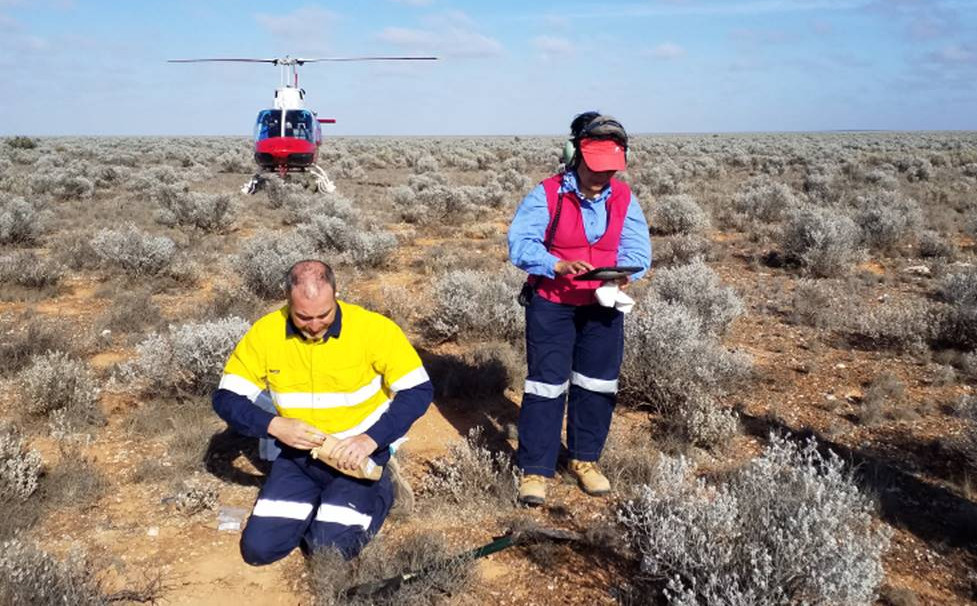
\includegraphics[width=1\textwidth,height=0.45\textheight,keepaspectratio]{%
figure/image002.jpg}
\caption{CSIRO Sampling by helicopter.}

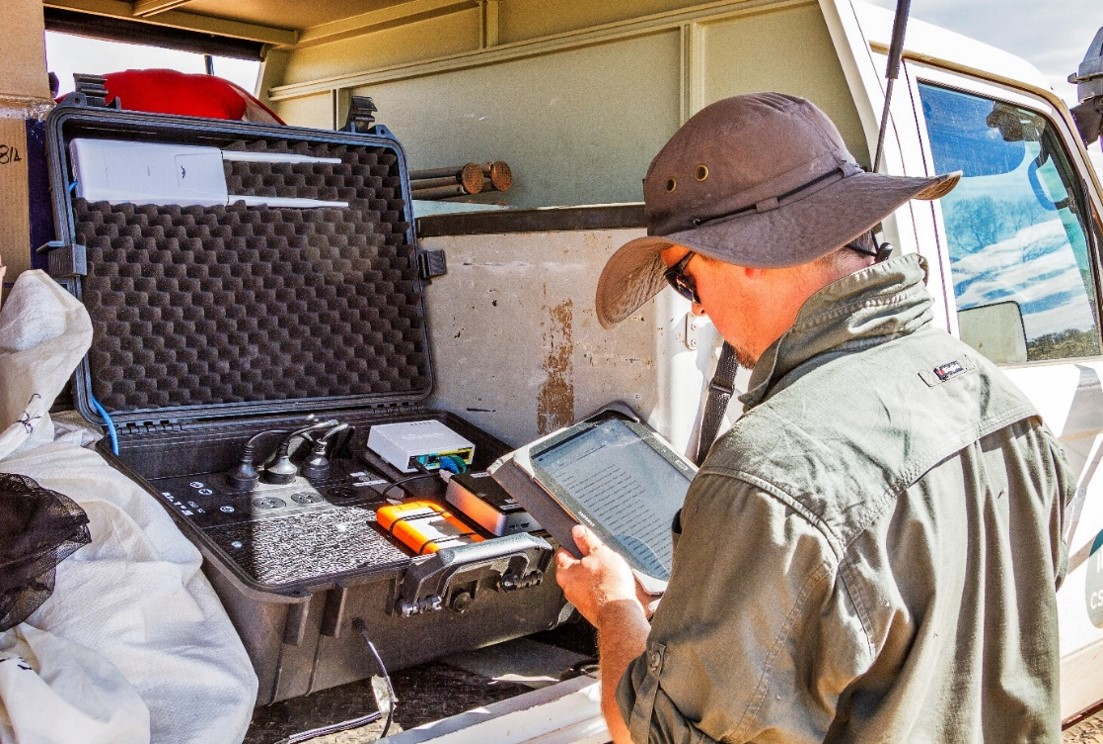
\includegraphics[width=1\textwidth,height=0.45\textheight,keepaspectratio]{%
figure/FAIMS_in_a_Truck.jpg}
\caption{CSIRO deployed a FAIMS server.}
\end{figure}
\end{column}
\end{columns}



   
\end{frame}

\begin{frame}
\parbox{\linewidth}{
FAIMS 3.0 retains the core functionality of FAIMS 2.5 and the idea of using a platform to generate custom offline data collection systems, but it represents a fundamental redesign, offering key performance, scalability, and user experience improvements:

\begin{itemize}
\item Compiled instead of interpreted: every custom collection system (module) will be its own app.
\item Cross-platform support: Android, iOS, and web.
\item Serverless(ish): Reduce the amount of equipment needed in the field through mesh network support.
\item GUI based designer: generates the XML-based domain specific language (DSL) code needed to customise a module.
\item A fully open source tile-based mapping service.
\item Export API: Allow external programs to interact with data in apps generated by the platform.
\end{itemize}
  }
\end{frame}

\mysection{challenge}


\begin{frame}\label{\secvariable}


  \begin{columns}[onlytextwidth]
  \begin{column}[c]{0.30\textwidth}
\begin{figure}


\includegraphics[width=1\textwidth,height=0.25\textheight,keepaspectratio]{%
figure/challenge_full_logo.png}
\vspace{12 pt}

\includegraphics[width=1\textwidth,height=0.25\textheight,keepaspectratio]{%
figure/USGS.jpg}
\vspace{12 pt}

\includegraphics[width=1\textwidth,height=0.25\textheight,keepaspectratio]{%
figure/bor_logo_2.jpg}
\vspace{12 pt}
\caption{Challenge text at: \\  \url{perma.cc/V8GZ-JF3Q}}

\end{figure}
\end{column}
  \begin{column}[c]{0.65\textwidth}

\parbox{\linewidth}{



``Data collection and capture are fundamental to water and environmental science and management.''

``[E]xisting apps do not provide the functionality and flexibility needed to support the broad range of water and environmental monitoring needs.''

``The Bureau of Reclamation, in collaboration with the U.S. Geological Survey ... [wants a] ... framework to support electronic data collection and capture using mobile devices across a diverse range of data collection situations.''
}
\end{column}

\end{columns}


\end{frame}
\begin{frame}
\parbox{\linewidth}{
The Data App's Challenge Stage 1 goals: A proposed design to hit the following objectives

\begin{itemize}
\item ``Development of a flexible, extensible, and open source data collection app framework will facilitate the use of mobile devices for field data collection.''
\item ``Standardize data collection practices ... , improve data collection efficiency, lower data collection costs, and ultimately improve data quality, transparency, and dissemination ...''
\item Tablets and smartphones in a flexible and extensible architecture for broad range of situations
\item Mandated full use of OSS to make it: ``substantially easier for any ... [community] to develop and share custom features to support agency-, program-, and community-specific protocols and standards for data collection, management, and sharing.''
\end{itemize}
}
\end{frame}

\mysection{solution}
\begin{frame}\label{\secvariable}
\begin{columns}[onlytextwidth]
	\begin{column}[c]{0.50\textwidth}
\parbox{\linewidth}{

Our proposed solution:

\begin{itemize}
\item Model-View-Controller design
\item A compiled native app on each platform from a single DSL specification.
\item A cross-complier like flutter.io or React to reduce coding load. 

\end{itemize}
}
\end{column}
\begin{column}[c]{0.45\textwidth}
\begin{figure}
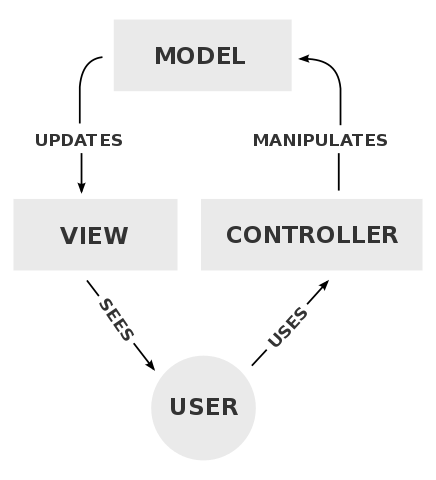
\includegraphics[width=1\textwidth,height=0.9\textheight,keepaspectratio]{%
figure/mvc.png}
\caption{Credit: Wikipedia}
\end{figure}
  \end{column}

\end{columns}


\end{frame}
\begin{frame}[t]
\begin{columns}[onlytextwidth]
	\begin{column}[c]{0.50\textwidth}
\parbox{\linewidth}{

Networking, sync, database:

\begin{itemize}
\item Mesh networking to allow for opportunistic updates \textit{in the field} instead of at basecamp.
\item Let's Encrypt automatic ssl.
\item Graph datastore
\begin{itemize}
\item CouchDB
\item PouchDB
\item The Multi-master Couch Replication Protocol
\end{itemize}
\end{itemize}
}
\end{column}
\begin{column}[c]{0.45\textwidth}
\begin{figure}

\vspace{12pt}
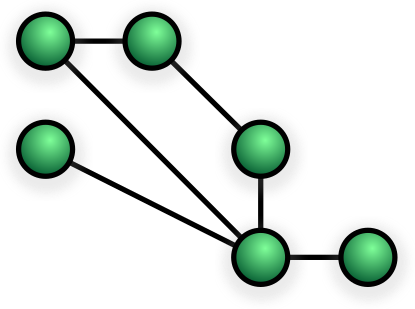
\includegraphics[width=1\textwidth,height=0.5\textheight,keepaspectratio]{%
figure/mesh.png}\\

\includegraphics[width=.45\textwidth,height=0.3\textheight,keepaspectratio]{%
figure/couchDB.png} \hspace{1mm} 

\includegraphics[width=.45\textwidth,height=0.3\textheight,keepaspectratio]{%
figure/pouchdb.png}
\vspace{12 pt}
\caption{Credit: Wikipedia and Apache}
\end{figure}
  \end{column}

\end{columns}


\end{frame}
\begin{frame}[c]
\parbox{\linewidth}{

Mapping and other essential features:

\begin{itemize}
\item Leaflet JS tile visualisation. Capable replacement of the GIS subsystem with geospatial actions done programmatically.
\item Roundtrip data exchange with desktop / online software through well defined csv and shp files for fast tabular editing and review.
\item Specific data collection methodologies can be distributed through Google Play and iTunes.
\item OSS TotalStation libraries for easier TS support.
\item OSS vector drawing and sketching.

\end{itemize}
}


\end{frame}

\mysection{oss}
\begin{frame}\label{\secvariable}
\parbox{\linewidth}{
OSS Technologies are a requirement of the Bureau of Reclamation DataApp challenge.

\vspace{12 pt}

Almost all of FAIMS 2.5 was OSS, save for our GIS library. It is (mostly) the expense of updating our GIS library that is forcing us to declare the old version as ``End-of-life.'' We are committed to avoiding this outcome in the future and ensuring a fully open platform.

\vspace{12 pt}

These DSL-defined and compiled apps can form an auditable centrepoint for reproducible science. By ensuring we produce OSS middle stages, the apps can be published and audited according to increasingly emphatic rules (See Nature's rules at: \texttt{https://perma.cc/3LX8-DYW7}) and published on (e.g.) osf.io. 
}
\end{frame}
\begin{frame}
\parbox{\linewidth}{
Planned OSS technologies:

\begin{itemize}
\item CouchDB \& PouchDB
\item LeafletJS
\item GDAL, OGR, Proj4, and Spatialite (as we still will need to do GIS computations in the backend)
\item Let's Encrypt (OSS and written in GO, but hosted by them.)
\item flutter.io
\item Completely OSS backend and Domain Specific Language processors
\item Graphviz for automatic diagram generation
\end{itemize}
}
\end{frame}

\begin{frame}
\parbox{\linewidth}{
Popular and useful research-specific capabilities from FAIMS Mobile will be retained and improved: 

\begin{itemize}
\item Defaults, flow logic, hierarchical selections, dynamic UI;
\item multilingual support using a plain-text localisation file;
\item on-device and server-side data validation;
\item aids to good practice including contextual HTML help, ``picture dictionaries'' and hierarchical selection trees that can guide users through complex processes;
\item embedding of URIs into form elements to link them to shared vocabularies, or ontologies, promoting data interoperability;
\item ``annotation'' and ``certainty'' metadata attached to every variable record.
\end{itemize}
}
\end{frame}

\mysection{CSIRO}
\begin{frame}\label{\secvariable}
\parbox{\linewidth}{
CSIRO Plans to use FAIMS 3.0:

\begin{itemize}
\item Add new modules for use of FAIMS in laboratories and field camps
\item Add new server options for different network bandwidths (full|low|no connectivity)
\item Sync across multiple servers for large-scale research involving many teams
\item Develop support for additional external sensors / devices
\item Include FAIMS in Active Sampling package for adaptive, data-driven sampling campaigns
\end{itemize}
}
\end{frame}

\begin{frame}[t]
\parbox{\linewidth}{%
\scriptsize
\nocite{Ballsun-Stanton2018-zd, Sobotkova2016-mx, Ross2015-ph, Ross2013-hi, Sobotkova2015-gm}
\bibliographystyle{abbrvnat}
\vskip-0.35cm
\bibliography{faims} 

Slides and \TeX~are available at \url{https://www.overleaf.com/read/qqgtqsnftwkj}
}
\end{frame}



\end{document}
